
\begin{figure}[ht]
	\centering
	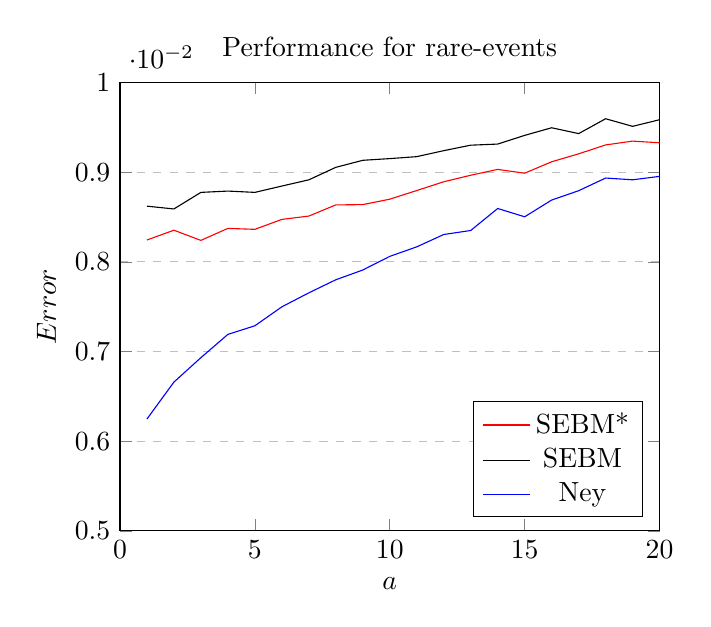
\begin{tikzpicture}[scale=1.0]
		\begin{axis}[
			title={Performance for rare-events},
			xlabel={$a$},
			xmin=0, xmax=20,
			ymin=0.005, ymax=0.01,
			ymajorgrids=true,
			ylabel={$Error$},
			grid style=dashed,
			xticklabel style={/pgf/number format/fixed},
			legend pos=south east,
		]
		\addplot[color=red] coordinates {
		(1,0.00824303292213)(2,0.00835254460775)(3,0.00823889901958)(4,0.00837282775519)(5,0.00836224382102)(6,0.00847304546572)(7,0.00851017908833)(8,0.00863460077097)(9,0.00863804338539)(10,0.00869846985716)(11,0.00879500733656)(12,0.00889282803455)(13,0.00896565747936)(14,0.00903077609739)(15,0.0089882646374)(16,0.00911591098473)(17,0.00920413707689)(18,0.00930364609753)(19,0.00934625157477)(20,0.0093274509829)
		};
\addlegendentry{SEBM*}
		\addplot[] coordinates {
		(1,0.00862069641015)(2,0.00858955811405)(3,0.0087743808877)(4,0.00878901680047)(5,0.00877444275485)(6,0.00884487890096)(7,0.00891432838845)(8,0.00905367745213)(9,0.00913216007212)(10,0.00915117512012)(11,0.0091729326627)(12,0.00923976838734)(13,0.00930083022747)(14,0.00931320531153)(15,0.00941021263061)(16,0.00949516652951)(17,0.00942991982115)(18,0.00959562689618)(19,0.00951087083342)(20,0.00958483466397)
		};
\addlegendentry{SEBM}
		\addplot[color=blue] coordinates {
		(1,0.00624623729428)(2,0.00665878512663)(3,0.00693118423385)(4,0.00719049815418)(5,0.00728657163073)(6,0.0074977146605)(7,0.00765404831751)(8,0.00779979414445)(9,0.00790867351491)(10,0.00806086399739)(11,0.00816687885093)(12,0.00830452351902)(13,0.00834938001649)(14,0.00859465863069)(15,0.0085021791087)(16,0.00868887793215)(17,0.0087930307321)(18,0.0089343323971)(19,0.00891468625456)(20,0.00895299850251)
		};
\addlegendentry{Ney}
		\end{axis}
	\end{tikzpicture}
    \caption{Average error of three stratified random sampling methods for the uniform-Bernoulli data sets of Section~\ref{sec:dataset2}, plotted against success parameter $a$, across 20,000 rounds.}
	\label{biggraph3}
\end{figure}
